\providecommand{\main}{./report}
\documentclass[../main.tex]{subfiles}
\begin{document}


\section{Building a benchmarking pipeline}\label{section:pipeline}
% pipeline goals
To facilitate conducting a comprehensive experiment, an accompanying software pipeline is to be built. Such a pipeline must be able to run feature ranking methods, select feature subsets, and validate the quality of the feature subsets using some validation estimator. After both the feature ranking- and validation step, evaluation metrics have to be computed - assessing the performance of the feature ranking both directly- and indirectly. After the metrics have been computed, results should be stored either on-disk or be uploaded to the cloud, after which they should be made interpretable by visualizing them. Furthermore, because the `direct' evaluation of feature rankings is only possible when a ground-truth reference of the relevant features exists (Section~\ref{section:evaluation-apriori-knowledge}), it is also desired to be able to generate synthetic datasets built in to the framework. In this way, a practitioner using the pipeline can easily design synthetic datasets suited for the purpose at hand.

% pipeline challenges
\textbf{Challenges} lie mainly in the scalability of the system. To conduct an experiment of moderate size, a single machine can be used for all stages of the pipeline: run the algorithms, collect and visualize the data. In such a small-scale context, the data- collection and visualization stage could as well be manual- no huge amounts of data have to be processed, so such a collection- and visualization stage could be run from a single script. When a larger experiment is desired to be run, however, a more sophisticated system is desired. Practitioners must not be restricted in running the pipeline on a single CPU or single machine, i.e., the system should support both \textit{horizontal}- and \textit{vertical} scaling. To design a system that can run experiments in such \textbf{scalable} and distributed ways, the system must be modular to facilitate distributing jobs over multiple machines, although it is also necessary to aggregate results of individual jobs as part of a pipeline step itself - requiring a piece of code to be aware of every job having finished.

% challenges -> this pipeline
An \textbf{implementation} of such a pipeline was made in Python, for the purposes of this paper. Many of the challenges described above were addressed and overcome by using an architecture that was built from the ground up to be scalable. Both the data- collection and aggregation processes were automated - after having run the pipeline for a collection of feature ranking methods and datasets, results are automatically stored, aggregated, and visualized. In this chapter, the reader is explained the general architecture of the system and the components that make the system work - after which the usage of the pipeline is shown along with its capabilities for scaling. The chapter is meant to be explanatory at first and provide concrete instructions and examples afterward.




% ARCHITECTURE
\subsection{Architecture}
To first get an idea of the structure of the system, comments are made on its architecture. The pipeline has two main components: an encapsulating pipeline `run' script and the pipeline itself. The pipeline run script is to be called the \textit{main} script: allowing us to differentiate easily between the two. Whilst the main script is designed to be generic and work for any \gls{ml} related benchmarking task, the pipeline itself is to be tailor made for the specific task at hand. Ideally, one could swap out the pipeline for another (custom built) one, but still using the main script mechanics: allowing a practitioner to create various but related tasks using a single framework.



\subsubsection{The main script}\label{section:pipeline-main-script}
The sole purpose of the main script is to do three things: (1) load a dataset, (2) split the dataset using a \gls{cv} method and lastly (3) run the pipeline. In this procedure, any dataset is loaded into the system using an \textit{adapter} - allowing data to come in from any source by use of a plug-able architecture (Section~\ref{section:pipeline-components-datasets}). Immediately after the dataset has been loaded a \gls{cv} split is conducted. In this way, because the cross-validation step is separated from all the pipeline steps itself, it is less likely that a pipeline can go faulty on the \gls{cv} process - since the data splitting operation was already conducted once a pipeline implementer gets their hands on the data. An illustration of the main script, with as part of it the pipeline, can be seen in Figure~\ref{fig:schematic-main-architecture}.

\begin{figure}[ht]
    \centering
    % https://docs.google.com/drawings/d/11qgqcMbxe6vyU8cv9KAZLeJPodVBi64TQCDwtNJp09g/edit
    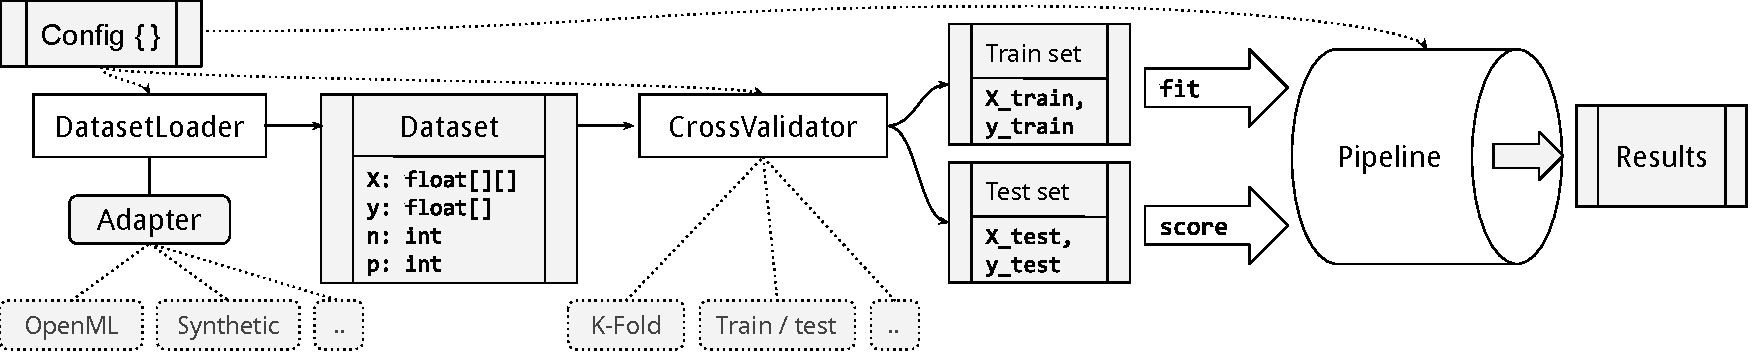
\includegraphics[width=\linewidth]{report/images/schematic-main-architecture.pdf}
    \caption{A general architecture schematic of the built benchmarking pipeline's \textit{main} script: providing data and instructions to the pipeline. Once the designated dataset is loaded using a configured adapter, the data is fed to the pipeline after a \gls{cv} split. The pipeline is first fit using the training data and then scored using the testing data, after which the results are collected and stored.}
    \label{fig:schematic-main-architecture}
\end{figure}

% config object
An important facet facilitating the operations in the main script is the \textbf{config} object (as seen at the top-left in Figure~\ref{fig:schematic-main-architecture}). The config object contains all configuration and parameters relevant to all pipeline steps, essentially storing all instructions required to perform a single pipeline run. It is thereby important to store \textbf{all} configuration and not to leave any parameters set at random or use temporary variables - the pipeline execution is desired to be \textit{deterministic} and therefore making its results \textit{reproducible}. In this way, experiments conducted using the pipeline are better suited for scientific experiments - a situation in which a user desires to be able to store exactly the state that produces a certain result and explain its findings in minute detail.

% hydra
To facilitate configuring the system in such a way, several options exist in the Python ecosystem. One could use the built-in \texttt{optparse} module, or its Python 3 counterpart \texttt{argparse}. The built-in packages leave much room for improvement, however. The modules do not allow loading config from a file, do not allow nesting, has only basic input validation and provides no tools for more complex configuration scenarios like the pipeline at hand. A solution for this is the \textit{Hydra} library \citep{yadan_hydra_2019}, a framework providing powerful utilities for configuring a Python application. The package allows one to create hierarchical and composable configurations, to be set using either the command-line or using yaml files. A simple yaml definition configuring the main script to use the `Iris Flowers' dataset and perform a K-fold \gls{cv} can be seen in Listing~\ref{code:pipeline-main-config}.

\begin{lstlisting}[caption={A simple configuration for the main script, using the `Iris Flowers' dataset and K-fold \gls{cv}.}, label={code:pipeline-main-config}]
defaults:
  - base_config
  - base_rank_and_validate
  - dataset: iris
  - cv: kfold
  - callbacks:
    - wandb
  - storage_provider: wandb
\end{lstlisting}

It can also be observed, in Listing~\ref{code:pipeline-main-config}, that there exist configuration possibilities for `callbacks' and a `storage provider'. These allow customizing a back-end for sending the result data to and an adapter for storing- or caching pipeline steps, respectively. Callbacks and the storage provider will be elaborated upon in Section~\ref{section:pipeline-callbacks} and Section~\ref{section:pipeline-storage-provider}, respectively. First, a look is taken at the pipeline implementation for feature ranking and subset validation, which is called \textit{Rank and Validate}.




\subsubsection{The `Rank and Validate' pipeline}\label{section:pipeline-rank-and-validate}
With the main script now defined, a better look can be taken at the pipeline implementation itself. Whereas the main script was still a general-purpose \gls{ml} benchmark runner, an implementation of the system by means of a pipeline is task-specific. i.e., one such pipeline is meant to execute a specific \gls{ml} task, such as performing evaluation on a feature ranker. The pipeline does so in a couple steps:

\begin{enumerate}
    \item \textbf{Resample} the dataset. Using the configured settings, the dataset is resampled. Options that are ought to be supported are shuffling, and more importantly; bootstrapping. It is thereby important to fixate a random `seed', which allows one to reproduce the resampling exactly.
    \item \textbf{Rank} features. Next, the feature ranker is set to work. The resampled data is passed to the ranker's \texttt{fit} function, after which the stored ranker might be cached.
    \item \textbf{Validate} feature subset. Finally, after the ranker has been fit, its ranking is used to validate its feature subsets, using some validation estimator. Again, the fit validation estimator might be cached. The final results are stored to disk and/or uploaded to the cloud.
\end{enumerate}

This process is illustrated in Figure~\ref{fig:schematic-pipeline-architecture}.

\begin{figure}[ht]
    \centering
    % https://docs.google.com/drawings/d/103YO-SX4JcwK_DbdT6G365ffvHJ7xCJQGaoUMoSvpeg/edit
    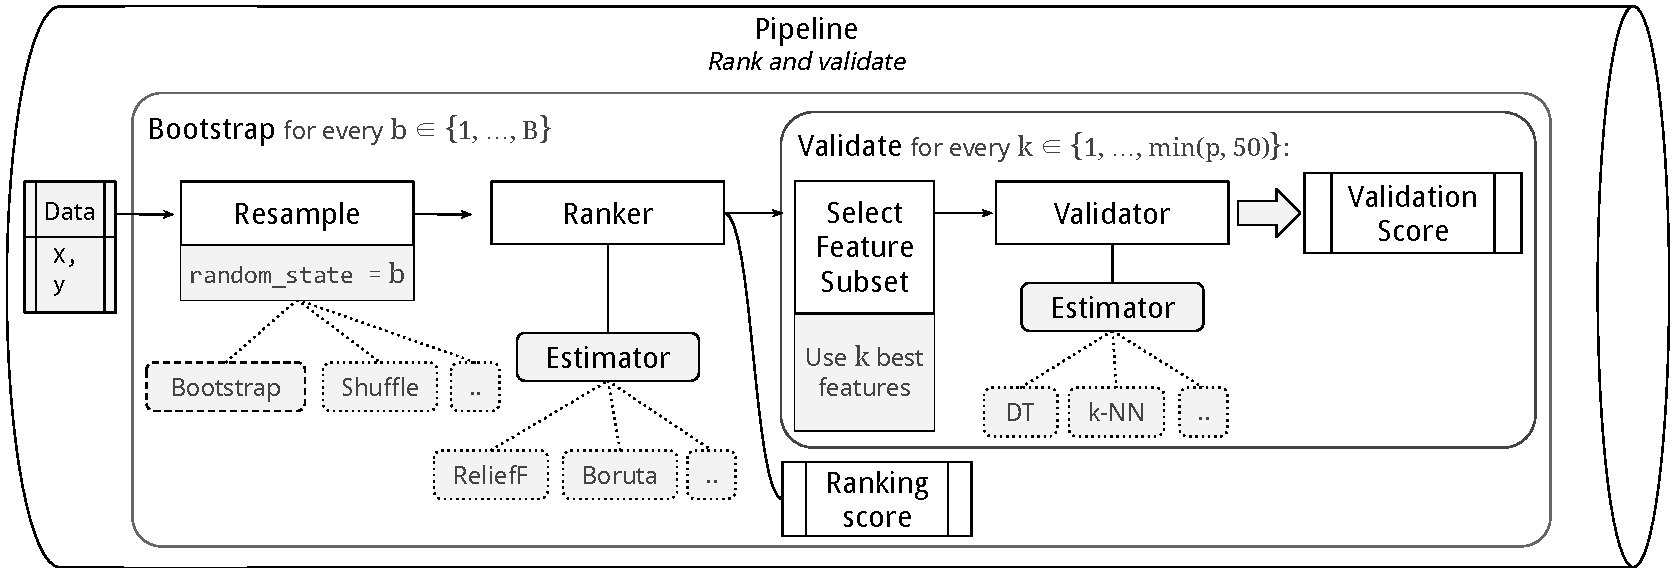
\includegraphics[width=\linewidth]{report/images/schematic-pipeline-architecture.pdf}
    \caption{The `Rank and validate' pipeline. The pipeline performs feature ranking, subset selection and subset validation, in a sequence of loops, such to facilitate bootstrapping. The pipeline is first fit and then scored.}
    \label{fig:schematic-pipeline-architecture}
\end{figure}

As can be seen illustrated by rectangles in Figure~\ref{fig:schematic-pipeline-architecture}, the above steps are executed in a specific sequence of loops. First of all, all steps (1-3) are passed through \textbf{twice}: once for the training data using the \texttt{fit} function and once using the testing data using the \texttt{score} function. The reasoning behind the division into these two steps is to force keeping application logic separate, i.e., to enforce a separation of concerns. Because the fitting step is essentially different than the scoring step, it makes sense to separate them. This separation also allows better implementations of caching, because a practitioner is enforced to store all estimator related state inside the instance itself. This distinction is on par with the sci-kit learn \citep{pedregosa_scikit-learn_2011} API.

For each of the two passes, the entire process is run $B$ separate times: once for each \textbf{bootstrap}. The random resampling seed is changed with each bootstrap iteration accordingly: making sure each bootstrap dataset is a different random resampling of the dataset, but yet keep the pipeline to be reproducible. The results from each bootstrap are then stored with each bootstrap random state attached, allowing a practitioner to differentiate between results and possibly aggregate- and group them.

Finally, each of the bootstrap iterations performs a number of feature subset validations. Ideally, in the case where a dataset has $p$ dimensions and a ranker has computed a feature importance score for each of them, it would be desired to validate $p$ feature subsets - the first subset starting with only the best ranked feature and subsequently including lesser-ranked features. However, this would fast become computationally intractable: in the case where $p$ is of considerable size, the amount of feature subsets to validate becomes vast, fast. A compromise between the thoroughness and computational tractability is to only validate some number of the best feature subsets up to a certain dimension. The choice that is made in this paper is to validate at most 50 feature subsets and possibly less if $p < 50$. i.e., the $\min (p, 50)$ best feature subsets are evaluated. This means for every $k \in \{1,\ldots,\min (p, 50) \}$ the $k$ best features are used for subset validation.

The \textbf{scoring} process happens only after all estimators in the pipeline have been fit. Once the fitting phase is complete, the testing sets will be passed to the pipeline's \texttt{score} function. Each estimator gets the opportunity to generate some score given the testing dataset. Because both the rankers \textit{and} estimators are considered estimators in the system, a ranker will also get such scoring opportunity. More specifically so, rankers and validators are scored in the following ways:

\begin{itemize}
    \item \textbf{Rankers} are scored using the dataset ground-truth relevant features, if available. Thereby metrics as described in Section~\ref{section:evaluation-apriori-knowledge} are used: the \textbf{R\textsuperscript{2} score} and the \textbf{logistic loss}.
    \item \textbf{Validators} are scored like described in Section~\ref{section:evaluation-validation-estimators}. i.e., the scoring depends on the dataset task: the \textbf{R\textsuperscript{2} score} is used in the case of \textit{regression}, and the \textbf{accuracy} score is used in case of \textit{classification}.
\end{itemize}

That said, a general picture of the pipeline architecture and data flow is now obtained. The pipeline is, however, more complex. The pipeline supports multiprocessing, distributed computing, caching, and data visualization. Moreover, each pipeline component has very different functionalities and can be configured separately from the rest of the pipeline. Therefore, a look is taken into the separate pipeline components first in Section~\ref{section:pipeline-components}, to then take an in-depth view of the pipeline execution afterwards, in Section~\ref{section:pipeline-execution}. Finally, an elaboration is made on data visualization in Section~\ref{section:pipeline-visualization}.







% COMPONENTS
\subsection{Components}\label{section:pipeline-components}
Each pipeline component can be configured using their own yaml files and has a reasonable level of isolation with respect to its module structure. The main components are discussed briefly.



\subsubsection{Datasets}\label{section:pipeline-components-datasets}
The system allows using datasets from numerous sources, using \textit{adapters}. Adapters are designed to be generic interfaces for fetching data from any source, as long as it can be expressed in two matrices $\mathbf{X}$ and $\mathbf{y}$. Although some adapters are available built-in to the framework, new adapters can easily be configured. Any such adapter must only implement a \texttt{get\_data} function, which returns the two matrices $\mathbf{X}$ and $\mathbf{y}$, given a configuration object facilitated by Hydra (see Section~\ref{section:pipeline-main-script}). Such adapters can implement any logic that retrieves the data themselves, be it logic for loading a dataset from local disk or from an internet platform.

\textbf{OpenML} is one such platform. OpenML \citep{vanschoren_openml_2014} is a platform for sharing and organizing data, completely open to all. Due to the flexible adapter structure of the system, and thanks to the availability of a Python package providing interfacing support with the platform, an integration with OpenML was made possible. Using the interface, datasets are fetched from a remote and cached to disk once downloaded. In this way, a cached version of the dataset is used in subsequent requests - making sure a dataset is not unnecessarily downloaded again. Integration with the platform allows users of the pipeline to access a large library of datasets, varying in type and domain. The dataset library features both regression and classification datasets, and of various target types, i.e., both univariate and multivariate. Also, the platform has multiple existing benchmark suites that can be used, such as the OpenML-CC18 \citep{bischl_openml_2019}. An example definition of a configuration file for loading an OpenML dataset is to be found in Listing~\ref{code:pipeline-openml-example}.

\begin{lstlisting}[caption={A dataset config for loading the `Iris Flowers' dataset from OpenML.}, label={code:pipeline-openml-example}]
name: Iris Flowers
task: classification
adapter:
  _target_: fseval.adapters.OpenML
  dataset_id: 61
  target_column: class
\end{lstlisting}

It can be seen, in Listing~\ref{code:pipeline-openml-example}, that a `target' class can be defined. This is passed to Hydra, which in turn instantiates the class with the given configuration. This is one of the core features that makes possible the modular adapter architecture that is in place.

\textbf{Synthetic} datasets can also be generated using the modular adapter-structure in place. By viewing a synthetic data generator as yet another adapter, providing data given a configuration object, both real-world and synthetic datasets can be used and generated using a single interface. A straight-forward way to generate synthetic datasets is to use the sci-kit learn \texttt{datasets} module, which provides functions for drawing samples from a wide variety of distributions. Aside from generic generators, there also exists support for drawing from more specific distributions, such as `two interleaving half circles', an `S curve' or a `swiss roll' distribution.

Most interesting for the current purposes, however, are two functions for generating classification- and regression datasets, \texttt{make\_classification} and \texttt{make\_regression}, respectively. Besides allowing one to configure the amount of samples and dimensions to generate, one can also define the desired informative-, redundant-, repeated- and irrelevant features to generate. In this way, a ground-truth for the relevant features can be constructed. In the case of regression, one can also retrieve the coefficients, or weighting, for each feature which are to be approximated, i.e., the desired feature importance for each feature. This means that whilst in the case of classification one has access to a \textit{binary} ground-truth, an \textit{exact} measure of the desired feature importance can be retrieved in the case of regression. An example definition of a synthetic classification dataset can be found in Listing~\ref{code:pipeline-synthetic-example}.

\begin{lstlisting}[caption={A dataset config generating a synthetic dataset using the sci-kit learn \texttt{make\_classification} function.}, label={code:pipeline-synthetic-example}]
name: Synclf hard
task: classification
adapter:
  _target_: sklearn.datasets.make_classification
  class_sep: 0.8
  n_classes: 3
  n_clusters_per_class: 3
  n_features: 50
  n_informative: 4
  n_redundant: 0
  n_repeated: 0
  n_samples: 10000
  random_state: 0
  shuffle: false
feature_importances:
  X[:, 0:4]: 1.0
\end{lstlisting}

Worth noting in Listing~\ref{code:pipeline-synthetic-example} is the presence of a `feature\_importances' attribute. This is the exact definition of the ground-truth relevant features, used by the pipeline. The system allows one to define the feature importances as numpy-indexed selectors, operating on some matrix the same size as $\mathbf{X}$. Every instance and every accompanying dimension can have a specific ground-truth weighting, although for the current purposes only \textit{global} feature- ranking and selection are considered. In the example above, it can be seen that the first 5 features are defined to be equally relevant: and therefore all have a uniform weighting of 1.0.




\subsubsection{Cross-Validation}
The Cross-Validator can be configured to be any class that has a \texttt{split} function, taking in the matrices $\mathbf{X}$ and $\mathbf{y}$ and returning a generator. The generator must then be an iterator over the number of configured folds, with each split returning the designated training- and testing data. An example configuration for a 5-Fold \gls{cv} split can be seen in Listing~\ref{code:pipeline-cv-example}.

\begin{lstlisting}[caption={A config for 5-Fold \gls{cv}, with shuffling. The split is reproducible due to the fixed random seed.}, label={code:pipeline-cv-example}]
name: K-Fold
splitter:
  _target_: sklearn.model_selection.KFold
  n_splits: 5
  shuffle: True
  random_state: 0
  fold: 0
\end{lstlisting}

As is seen in Listing~\ref{code:pipeline-cv-example}, a \gls{cv} technique can be configured to be a sci-kit learn module. Another important thing to note is the fixed `fold' attribute, set in this case to 0. Because the pipeline always executes exactly one fold, performing a K-Fold \gls{cv} is done by executing the pipeline multiple times using different values of \texttt{fold}.




\subsubsection{Resampling}
Built in, there are two options for resampling. There exist options for (1) bootstrap sampling and (2) shuffle resampling. Whilst the latter only changes the permutation of the dataset, the former performs resampling \textit{with} replacement, therefore actually changing the dataset distribution. \textbf{Bootstrap} resampling is configured like as can be seen in Listing~\ref{code:pipeline-bootstrap-example}.

\begin{lstlisting}[caption={A config for bootstrap sampling using a sample size of 1.0, i.e, using the full dataset.}, label={code:pipeline-bootstrap-example}]
name: Bootstrap
replace: true
sample_size: 1.00
\end{lstlisting}

Noteworthy, in Listing~\ref{code:pipeline-bootstrap-example}, is the `sample size' parameter. If needed, the dataset can be down- or up-sampled. Although up-sampling generally does not make much sense, down-sampling can increase the stochasticity of the bootstrapped dataset permutation. This means that, if desired, one can create more `random' distributions by setting \texttt{sample\_size} to a lower number. Lastly, a random seed can be fixed, like as can be seen in the pipeline schematic, Figure~\ref{fig:schematic-pipeline-architecture}: the resampling \texttt{random\_state} is set to the bootstrap number. In this way, the resampling is exactly reproducible.




\subsubsection{Estimators}
In the context of the current system, an `estimator' can mean two things. An estimator is either: (1) a feature ranker or (2) a validation estimator. Still, the two are combined into a single estimator interface: which is because both can share much of the same API for interacting with them. Both implement a fitting- and scoring step, and can be of regressor- or classifier type. Also, to support these two learning tasks in a better way, any estimator is encapsulated in a generalized estimator interface. An example configuration for a \textbf{ranking} estimator can be seen in Listing~\ref{code:pipeline-estimator-example}.

\begin{lstlisting}[caption={An estimator config for ReliefF \citep{kononenko_estimating_1994}.}, label={code:pipeline-estimator-example}]
name: ReliefF
classifier:
  estimator:
    _target_: skrebate.ReliefF
regressor:
  estimator:
    _target_: skrebate.ReliefF
estimates_feature_importances: true
estimates_feature_support: false
\end{lstlisting}

Both a regressor and classifier were defined in a \textit{single} interface, as can be observed in Listing~\ref{code:pipeline-estimator-example}. Although the two were in this case defined to be the same, they might have as well pointed to different modules. Under the hood, the system detects the configured dataset task at initialization and instantiates either one of the two modules. Furthermore, the system has to be told the capabilities of the estimator, e.g., whether it estimates targets, feature importance or feature support. This is done using the boolean attributes starting with `estimates\_': where in this case the ReliefF estimator estimates just the feature importance, but no feature subset.

\textbf{Validation} estimators are configured in much the same way - and can also have both a regressor and classifier defined. The interface also allows indicating an estimator's support for \textit{multioutput} learning or the estimator requiring a \textit{strictly positive} dataset to work.





\subsubsection{Storage providers}\label{section:pipeline-storage-provider}
A \textit{storage provider} is defined to be a bridge between the pipeline and a file system, independent of whether this file system is on the local disk or in the cloud. Because in the pipeline it is desired that the fit estimators can be cached, a storage system must be built accordingly. Independent of exactly where the files are stored, a storage provider can be constructed by implementing routines for \textbf{saving} and \textbf{restoring} files. As long as the storage provider returns a usable file object given a file path, the system is ambivalent about how the file is loaded. A schematic of how this storage provider works is to be seen in Figure~\ref{fig:schematic-storage-provider}.

\begin{figure}[ht]
    \centering
    % https://docs.google.com/drawings/d/1fuHtYzybRbJQToTn9ct3ObY1xz9BHxc6Hsq17mq-Bbs/edit
    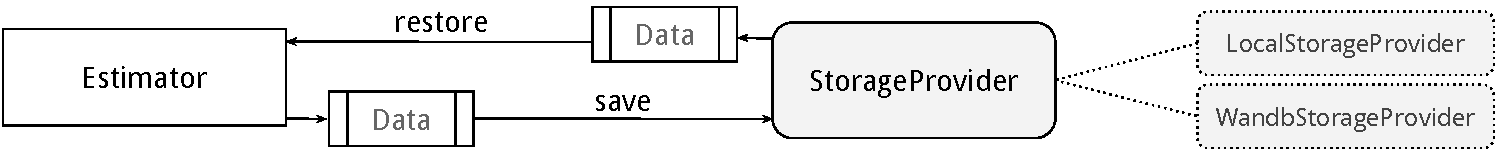
\includegraphics[width=\linewidth]{report/images/schematic-storage-provider.pdf}
    \caption{An illustration of the Storage Provider functionality. The storage provider can be used to save- and restore files, using both a local- or remote file system.}
    \label{fig:schematic-storage-provider}
\end{figure}

In the example in Figure~\ref{fig:schematic-storage-provider}, it can be seen that the storage provider is used by an estimator to save- and restore data. Such data can, for example, be a \textit{pickle} file used to serialize- and deserialize a fit estimator object.

\textbf{Caching} is supported in this way. By storing a reference to the file-path right in the job configuration itself, cached files can be reused via either the local- or remote file system. The pipeline allows configuring exactly \textit{which} parts of the pipeline allow using cached versions of their fit estimators, such that in any subsequent run of a job, some estimators can be reused and others overwritten. This functionality facilitates running multiple validation estimators given a single fit feature ranker, for example.

\subsubsection{Callbacks}\label{section:pipeline-callbacks}
The final component to discuss is the \textit{Callback}. A callback can be used to send data to a back end during the execution of the pipeline. Such data can be configurations, objects containing metrics or entire tables with results. The requirements for implementing such a callback are low, since any such data can be stored as an opt-in. If a pipeline user desires so, the usage of a callback can be completely ignored, storing only data to the disk using the storage provider. Sending metrics to a callback can, however, be a powerful way to send data to a database or cloud back-end right in the pipeline. In this way, the usual data collection phase can be automatized. About an implementation of such a callback can be read in Section~\ref{section:pipeline-visualization}. First, however, a closer look is taken at the pipeline execution and its scalability.





% EXECUTION
\subsection{Execution}\label{section:pipeline-execution}
The pipeline execution happens in a predefined number of steps. Because the pipeline is desired to be run in parallel and in a distributed way, the execution of such a system is nontrivial. Support for scaling in both the horizontal- and vertical directions are required, i.e., the pipeline must be able to scale over more machines but must also scale over more system resources such as CPU or RAM. Systems that fulfil such desires are \gls{hpc} systems, which are designed to support scalable computing \citep{ristov_superlinear_2016}. An elaboration is made on an implementation of such a scalable architecture.




\subsubsection{Multiprocessing}
To facilitate \textit{vertical} scaling, a multiprocessing implementation is built. It is thereby the goal to best utilize the system resources at hand: maximizing the usage of the available processors. To do so, certain iterative parts of the pipeline were wrapped in an encapsulating `Experiment' module. The task of the module is, then, to pick up wherever the pipeline would iterate over a number of steps, and add multiprocessing support. As could be read in Section~\ref{section:pipeline-rank-and-validate} and seen in Figure~\ref{fig:schematic-pipeline-architecture}, the pipeline has two main loops: the first (1) runs $B$ bootstraps and the second (2) validates $\min (p, 50)$ feature subsets. In this implementation, the choice was made to distribute the former loop, i.e., to distribute the bootstraps over multiple CPU's. An illustration making clear the functionality of such a multiprocessing approach can be seen in Figure~\ref{fig:schematic-pipeline-multiprocessing}.

\begin{figure}[ht]
    \centering
    % https://docs.google.com/drawings/d/1_6Z8nmHv9hQTTmM0f6SqOTsNDeNPfdl2hASd5M4cJFI/edit
    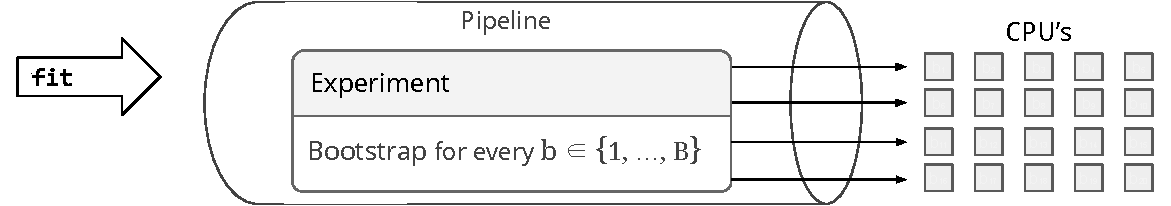
\includegraphics[width=0.8\linewidth]{report/images/schematic-pipeline-multiprocessing.pdf}
    \caption{The pipeline multiprocessing distribution process. In the pipeline fit step the set of bootstraps is distributed over the available CPU's.}
    \label{fig:schematic-pipeline-multiprocessing}
\end{figure}

As could be seen in Figure~\ref{fig:schematic-pipeline-multiprocessing}, every bootstrap resampling job is assigned to a processor. In case more bootstraps are to be run than the number of available processors, i.e., $B >$ \# CPU's, some CPU's are assigned more than one bootstrap resampling job. In \gls{hpc} environments, it is common to have a dozen CPU's available in a single job. Given that a reasonable but still feasible number of bootstraps to run is also a few dozen, it can be straight-forward option to configure the number of bootstraps to run as the number of CPU's available in a job on the designated \gls{hpc} environment.

% main thread to subprocess communication
Important to note in such a multiprocessing job, is the available \textit{scope} of variables accessible inside any subprocess. Because each subprocess runs isolated on a CPU, it cannot access variables exclusively available to the main thread process. In the case that such a subprocess requires access to variables from the main thread, either one of two options can be considered. One option is to pass down a copy of the variables in question to the subprocess: this, however, does not apply when such variables change during the program execution. In that case, the second option is to communicate between the subprocess and the main thread. In this way, functionality such as storing cache files (Section~\ref{section:pipeline-storage-provider}) can still be done in the main thread, if it is deemed necessary.




\subsubsection{Distributed computing}
To make the pipeline \textit{horizontally} scalable, an approach must be constructed for distributing the processes over multiple machines. Although running multiple jobs in a \gls{hpc} environment can be a relatively straight-forward practice, a choice must be made on the amount of processing to put in a single job. For example, if a system were in place that automatically distributes jobs over a number of processors and machines by itself, the horizontal- and vertical scaling approaches could be tackled in a single solution. In this scenario, an automatic job scheduler would assign very small jobs to nodes and processors by itself; the smallest experimental unit could be running one bootstrap on a single feature ranker. However, such an approach is rather complex and often unsupported by existing \gls{hpc} systems. Therefore, the choice is to go with a hybrid approach - a single \gls{hpc} job is assigned multiple experiments. In this way, long queue waiting times as a consequence of running many small jobs are prevented.

% Redis Queue
Such an approach can be accomplished by the use of a second job queue, next to the \gls{hpc} job queue. The queue of choice is \gls{rq}, a library for keeping track of an arbitrary number of job queues in Redis which then can be executed by \textit{workers}. Workers are run on the \gls{hpc} system itself and are built solely to execute work coming from the queues. The library is built to be fault-tolerant, scalable, and easy to use. The basic idea is that during the enqueueing phase, a piece of Python code is serialized into a binary format and stored in Redis into a First-In-First-Out queue. Then, once the time has come that the job can be executed, the job execution code is deserialized from Redis back into Python code, and executed. This functionality can be seen illustrated in Figure~\ref{fig:schematic-pipeline-redis-queue}.

\begin{figure}[ht]
    \centering
    % https://docs.google.com/drawings/d/1m1vOiICDB-7mi9qHqq7xBl9_mouTZoL2FEK8y3rag7I/edit
    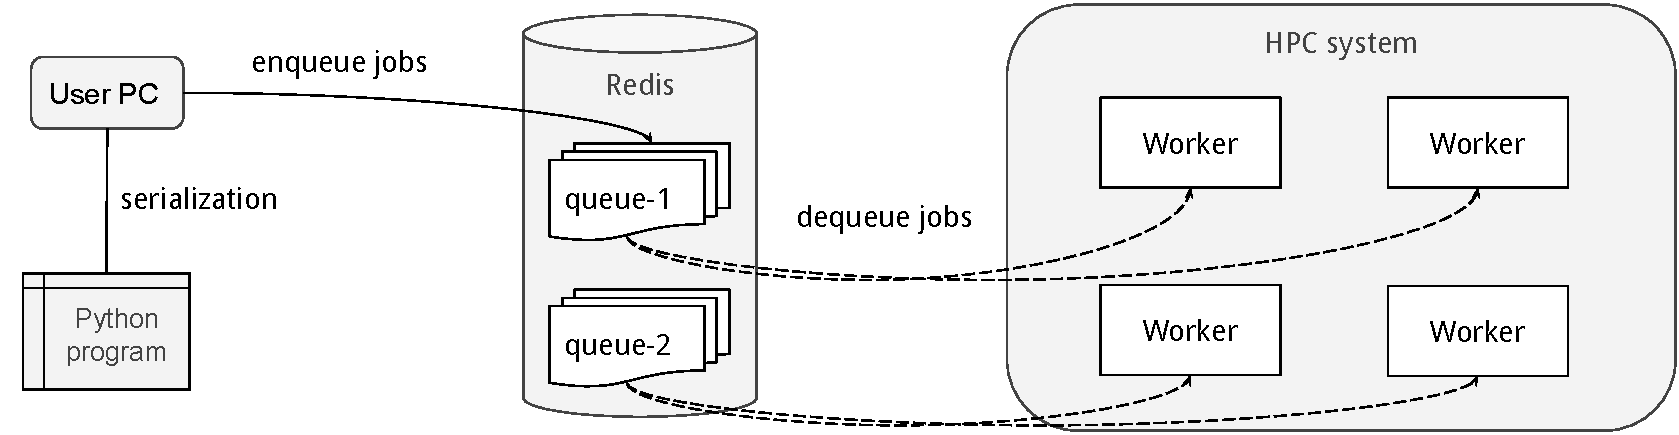
\includegraphics[width=\linewidth]{report/images/schematic-pipeline-redis-queue.pdf}
    \caption{The \gls{rq} enqueueing- and dequeueing process. Jobs are serialized on the client and stored in Redis FIFO queue. Workers on the \gls{hpc} system process the jobs on the designated queues.}
    \label{fig:schematic-pipeline-redis-queue}
\end{figure}

% benefits in using RQ
It can be seen in Figure~\ref{fig:schematic-pipeline-redis-queue}, that the Redis database acts as an intermediary between the user and the \gls{hpc} system. Whilst the queues in Redis may contain hundreds or thousands of jobs, the amount of jobs on the \gls{hpc} system only need to be several: one job for each worker. Each worker may run on its own node, or share a node by means of a virtual machine. In overall, the \gls{rq}-based approach has a number of benefits.

\begin{itemize}
    \item First of all, the \gls{hpc} system is not overloaded by small jobs. Instead, \gls{rq} is better designed to store and process a multitude of small jobs - preventing overhead and long queuing times in the \gls{hpc} system. This is because the only jobs that are launched on the \gls{hpc} system are the workers - which can be configured to last an arbitrary amount of time, or to terminate once its queue is empty.
    \item A second benefit is that \gls{rq} has good support for handling job failures. \gls{rq} allows automatically retrying failed jobs, with optionally set time intervals between tries, such that in the case of a network time-out or system error the job is be restarted without further human input. Furthermore, if the job still fails execution after its pre-configured number of retries were completed, the job is not just removed from all queues. Instead, the job is moved to a separate `failed job' queue. The error logs for jobs in this queue are easily inspected using a dashboard interface for \gls{rq}.
    \item A last benefit is the serialization- and deserialization process in \gls{rq}. Because Redis does not just store instructions to execute the code, but the actual execution code itself, code on the \gls{hpc} system might be changed during the time a job is in queue. This gives a practitioner more flexibility to change program code and run the pipeline at the same time.
\end{itemize}

% RQ Launcher
As a side benefit, the Hydra library used for configuring the system has built-in support for working with \gls{rq}. By use of a plugin, the pipeline can be configured to enqueue its jobs to \gls{rq} instead of executing right away. An important note is that due to the serialization process the Python version during enqueueing and dequeueing have to be exactly equal.






\subsection{Data- collection and visualization}\label{section:pipeline-visualization}
Finally, all results coming out of the pipeline should be collected and visualized. Since the pipeline has support for plugging in any arbitrary `Callback' (Section~\ref{section:pipeline-callbacks}), primitives are in place for sending the data to a data- collection and visualization back-end. Any such callback can implement functions for processing the pipeline configuration, individual metric objects, and result tables. Because the pipeline is built to be executed at scale, a clear distinction is made between the pipeline execution phase and the data collection phase: the two are separated by means of the \textit{Callback} interface.

One callback implementation is the `Wandb' callback, providing integration with the Weights and Biases platform \citep{biewald_experiment_2020}. Weights and Biases is a platform for real-time experiment tracking and visualization, with built-in primitives in Python. The platform allows you to upload tables, metrics, or configuration objects, and subsequently visualize them in the front-end interface. The platform also allows one to upload- and download raw files, allowing a user to integrate remote caching functionality (Section~\ref{section:pipeline-storage-provider}). A screenshot of the platform front-end can be seen in Figure~\ref{fig:pipeline-wandb-frontend}.

\begin{figure}[ht]
    \centering
    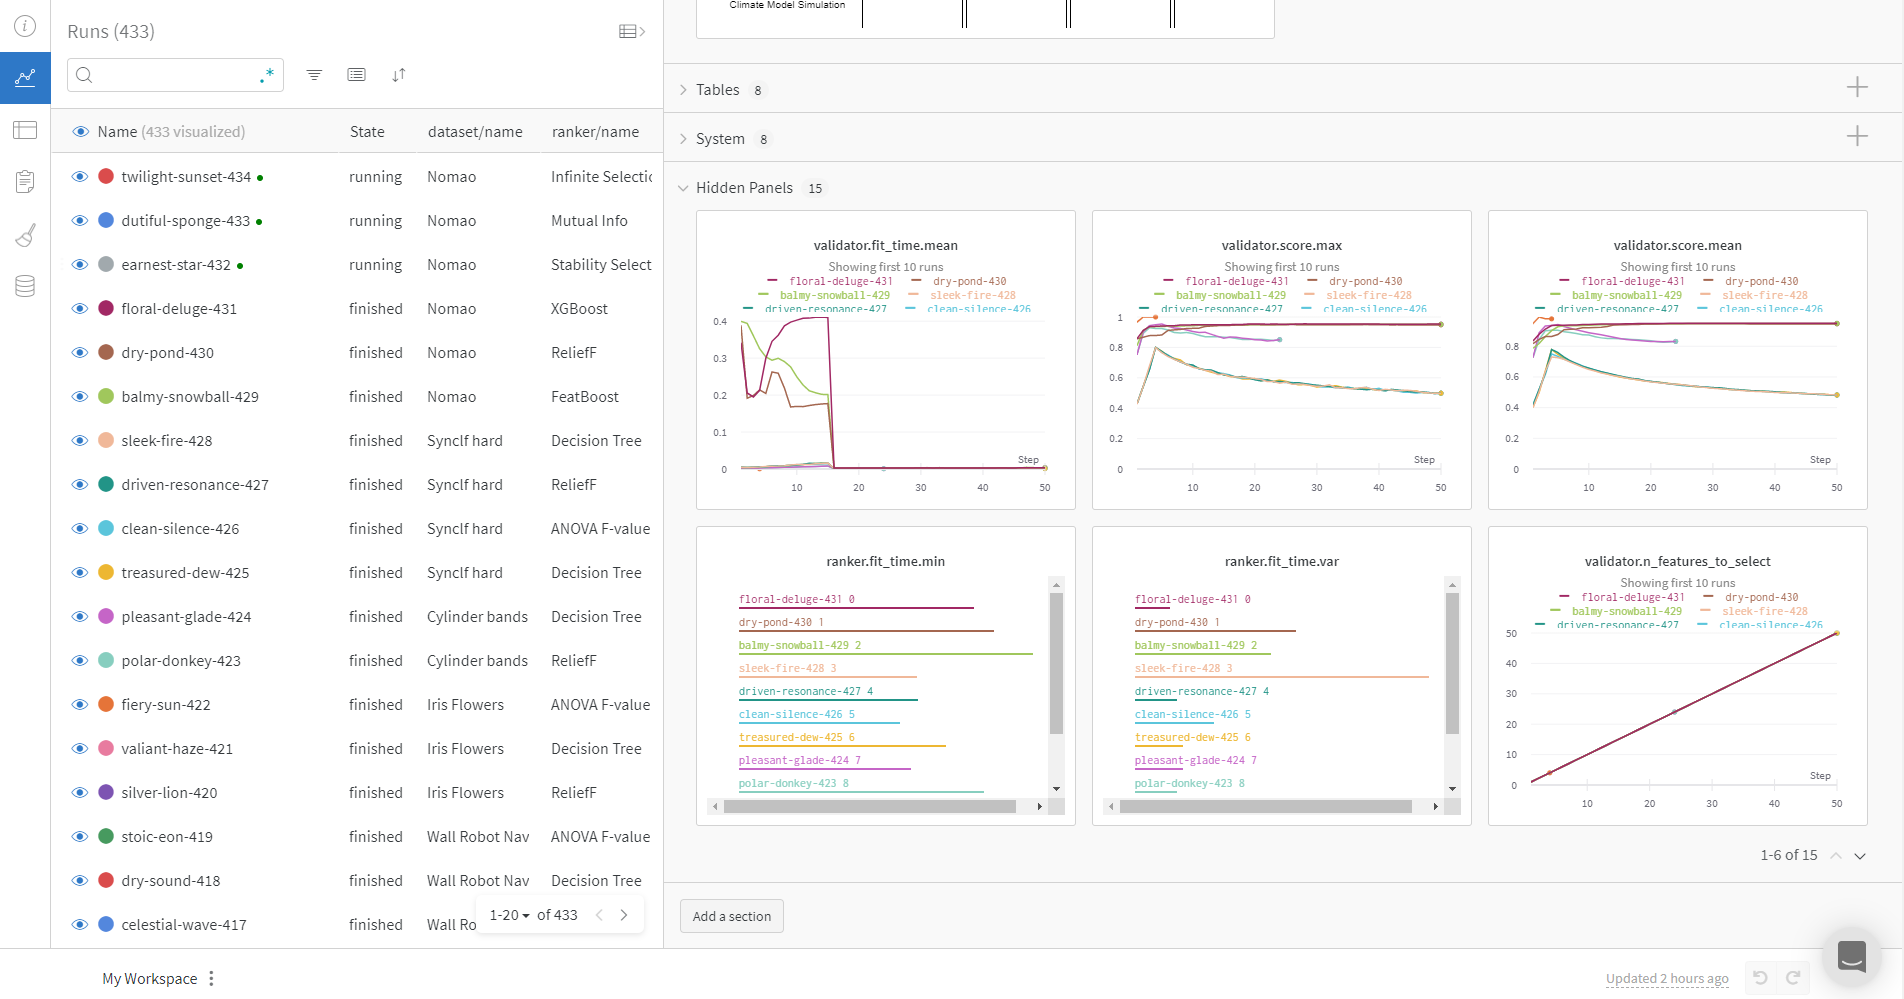
\includegraphics[width=0.9\linewidth]{report/images/pipeline-wandb-frontend.PNG}
    \caption{The Weights and Biases dashboard front-end. The platform allows tracking experiments, aggregating data, and visualizing results.}
    \label{fig:pipeline-wandb-frontend}
\end{figure}

An important feature on the Weights and Biases platform is the ability to collect- and aggregate data interactively in the front-end. This is done by means of `Vega-Lite' \citep{satyanarayan_vega-lite_2017}, a visualization grammar for creating interactive visualizations in a front-end environment. This allows a user to send `raw' data to the dashboard, and aggregate it on the front-end itself. Any aggregation operation can be applied, be it taking averages, sums or computing the variances. The front-end then allows you to visualize the aggregated data using a simple grammar. In this way, the pipeline requires much less small adjustments and modifications for the user to be satisfied with the data aggregation process - the data can be summarized in a later stage after all results are already in.



\biblio
\end{document}
